\documentclass[class=report, crop=false, 12pt,a4paper]{standalone}
\usepackage{enumitem}
\usepackage{multicol}
\usepackage{graphicx}
\usepackage{float}
\usepackage{amsmath}
\usepackage{amssymb}
\usepackage{mathtools}
\usepackage{siunitx}
\usepackage{commath}
\usepackage{array}
\usepackage{natbib}
\usepackage{cancel}
\usepackage[a4paper,width=150mm,top=25mm,bottom=25mm]{geometry}
\setlength{\parindent}{0pt}
\begin{document}
\section{Thick wall cylinders}
Lame's equations
\begin{align}
    \sigma_r &= \frac{p_i r_i^2 - p_or_o^2}{r_o^2 - r_i^2} - \frac{\left(p_i-p_o\right)r_i^2 r_o^2}{\left(r_o^2 - r_i^2\right)r^2}\\
    \sigma_{\theta} &= \frac{p_i r_i^2 - p_o r_o^2}{r_o^2 r_i^2} + \frac{\left(p_i-p_o\right)r_i^2 r_o^2}{\left(r_o^2 - r_i^2\right)r^2}
\end{align}
We have seen that a thick cylinder subjected to internal pressure experiences very high peaks of stress at the inner surface. 
\begin{figure}[H]
    \centering
    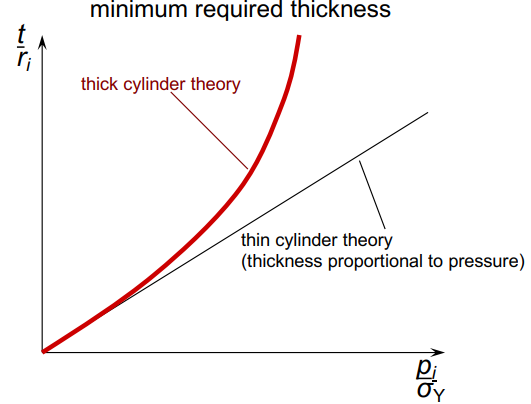
\includegraphics[height = 5cm]{../img/diagram118.png}
    \caption{The required thickness increases non-linearly with the pressure.}
\end{figure}
The design of cylinders that have to maintain high levels of pressure requires specific strategies. aimed at reducing the hoop stress levels at the inside surface.
\begin{figure}[H]
    \centering
    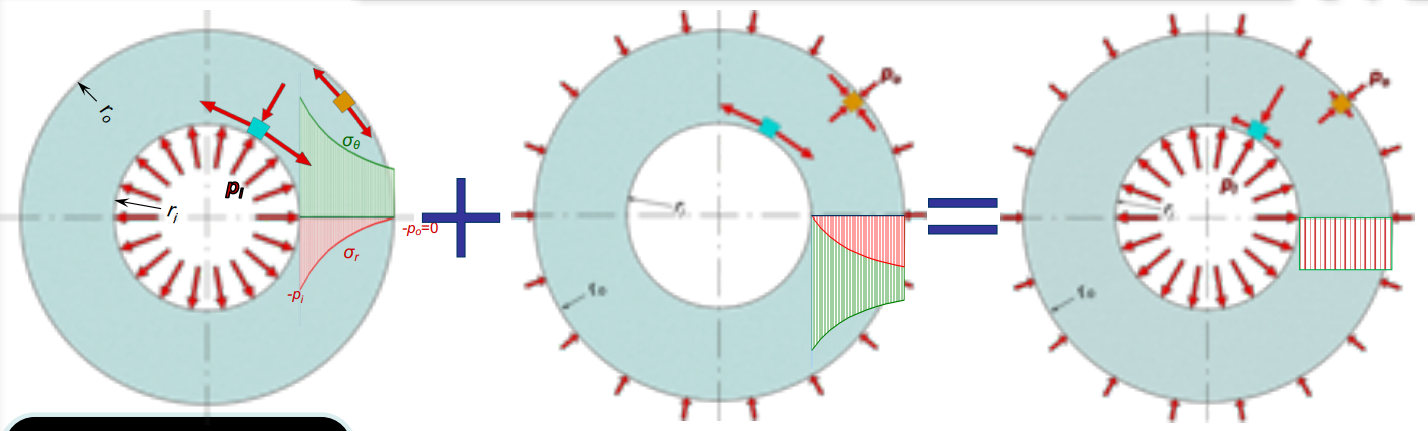
\includegraphics[width = \textwidth]{../img/diagram119.png}
    \caption{}
\end{figure}
A possible solution could be reducing the level of hoop stress by increasing the pressure at the outer surface.
\section{Compound cylinders}
\subsection{Containing high pressures}
This can be done by shrinking another tube on the outside of the original one:
\begin{figure}[H]
    \centering
    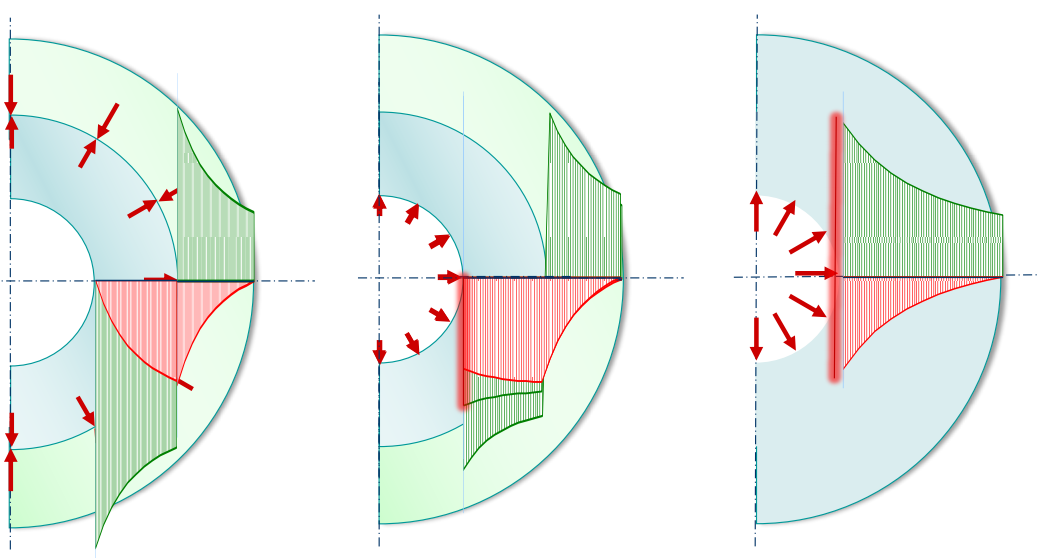
\includegraphics[width = \textwidth]{../img/diagram120.png}
    \caption{}
\end{figure}
\subsection{Compound or 'built-up' cylinders}
THis compound (or built-up) arrangement is obtained by assembling two cylinders with initial diametrical interference $\delta$ at room temperature. The outer cylinder is heated and the inner cylinder is cooled, in order to compensate for the interference by thermal expansion/contraction and allow assembly. Returning the components to room temperature, a set of residual radial and hoop stress is introduced, which locks the two components firmly together. 

The interference between the two cylinders will produce an external pressure $p_{int}$ acting on the internal cylinder, and an equal internal pressure $p_{int}$ acting on the external cylinder, function of the interference $\delta$. 

\begin{figure}[H]
    \centering
    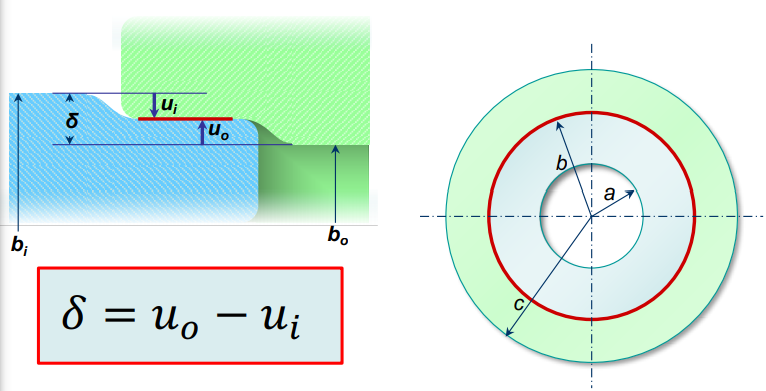
\includegraphics[height = 5cm]{../img/diagram121.png}
    \caption{}
\end{figure}

Interface pressure can be expressed as a function of the interference, by using the solid mechanics equations.
\subsubsection{Other applications}
\begin{figure}[H]
    \centering
    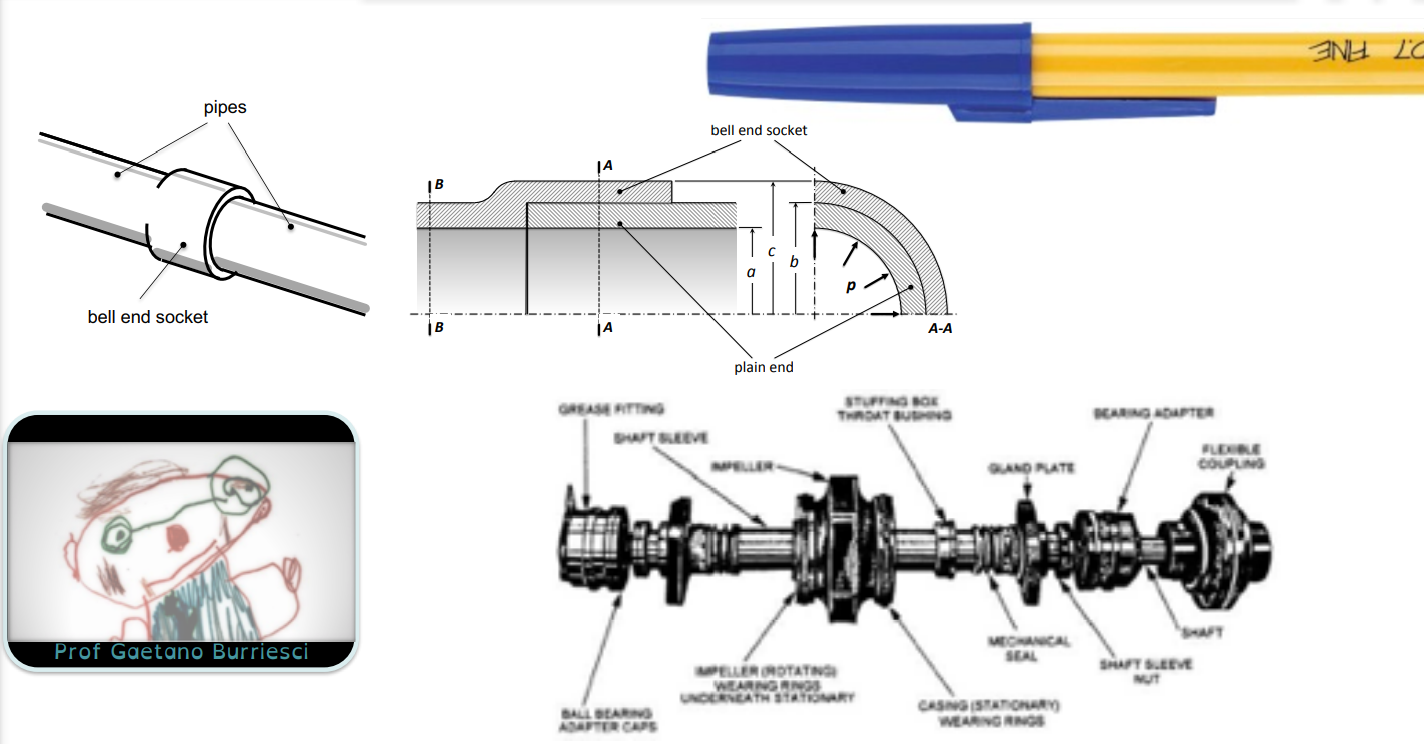
\includegraphics[width = \textwidth]{../img/diagram122.png}
    \caption{}
\end{figure}
\subsection{Stress state at the interface}
\begin{gather}
    u = \frac{r}{E}\left(\sigma_{\theta} - v \sigma_r\right)\\
    \rightarrow u_i = \frac{b}{E_i}\left[\sigma_{\theta, i} \left(b\right) - v_i \sigma_{r,i} (b)\right]
\end{gather}
Lame's equations:
\begin{gather}
    \sigma_r = A - \frac{B}{r^2}\\
    \sigma_{\theta} = A + \frac{B}{r^2}
\end{gather}
Boundary conditions:
\begin{gather}
    \sigma_{r,i}(a) = 0 = A - \frac{B}{a^2}\\
    \sigma_{r,i}(b) - -p_{int} = A - \frac{B}{b^2}\\
    A = -p_{int}\frac{b^2}{b^2 - a^2}\\
    B = -p_{int}\frac{a^2 \cdot b^2}{b^2 - a^2}
\end{gather}
Substituting:
\begin{equation}
    \sigma_{\theta,i} = A + \frac{B}{r^2} = -p_{int}\frac{b^2}{B^2 - a^2} \left(1 + \frac{a^2}{r^2}\right)
\end{equation}
Therefore:
\begin{gather}
    \sigma_{r,i}(b) = -p_{int} \hspace{1cm} \sigma_{\theta,i}(b) = -p_{int}\frac{b^2 + a^2}{b^2 - a^2}\\
    u_i = -p_{int} \frac{b}{E_i} \left(\frac{b^2 + a^2}{b^2 - a^2} - v_i\right)
\end{gather}
Repeating:
\begin{gather}
    u_o = \frac{b}{E_o}\left[\sigma_{\theta,o} (b) - v_o \sigma_{r,o}(b)\right]
\end{gather}
Lame's equations:
\begin{gather}
    \sigma_r = A - \frac{B}{r^2}\\
    \sigma_{\theta} = A + \frac{B}{r^2}
\end{gather}
Boundary conditions:
\begin{gather}
    \sigma_{r,o}(b) = -p_{int} = A - \frac{B}{b^2}\\
    \sigma_{r,o}(c) = 0 = A - \frac{B}{c^2}\\
    A = -p_{int} \frac{b^2}{b^2- c^2}\\
    B = -p_{int} \frac{b^2 \cdot c^2}{c^2 - b^2}
\end{gather}
Substituting:
\begin{gather}
    \sigma_{\theta,o} = A + \frac{B}{r^2} = -p_{int} \frac{b^2}{c^2 - b^2} \left(1+ \frac{c^2}{r^2}\right)
\end{gather}
Therefore:
\begin{gather}
    \sigma_{r,o}(c) = 0 \hspace{1cm} \sigma_{\theta,o}(b) = p_{int}\frac{c^2 + b^2}{c^2 -b^2}\\
    u_o = p_{int} \frac{b}{E_o}\left(\frac{c^2 + b^2}{c^2 - b^2} + v_o\right)
\end{gather}
\end{document}